\section{Methodology}
\label{Methodology}

Replace all this with your specific methodology that you used in your Software Testing research project.  The Methodology section explains how the research was conducted in detail. It provides a clear and precise description of the study design, data collection methods, tools or instruments used, and the procedures followed. This section also outlines the sampling techniques, participants or data sources, and any statistical or analytical methods applied. The goal of the methodology is to allow other researchers to replicate the study or understand how the results were derived. It should be detailed enough to ensure transparency and reproducibility while justifying why certain methods were chosen. 

\subsection{System Usablity Scale}
This section just shows that you can include figures very easily.  You first talk about the figure, then it follows.  For example, Figure~\ref{fig:sus} presents the System Usablity Scale that has been used in thousands of usabilty studies.  If you create figures, make sure to store them in the ``figures'' subfolder.  This will help keep everything in your \LaTeX  project more organized.

\begin{figure}
	\centering
	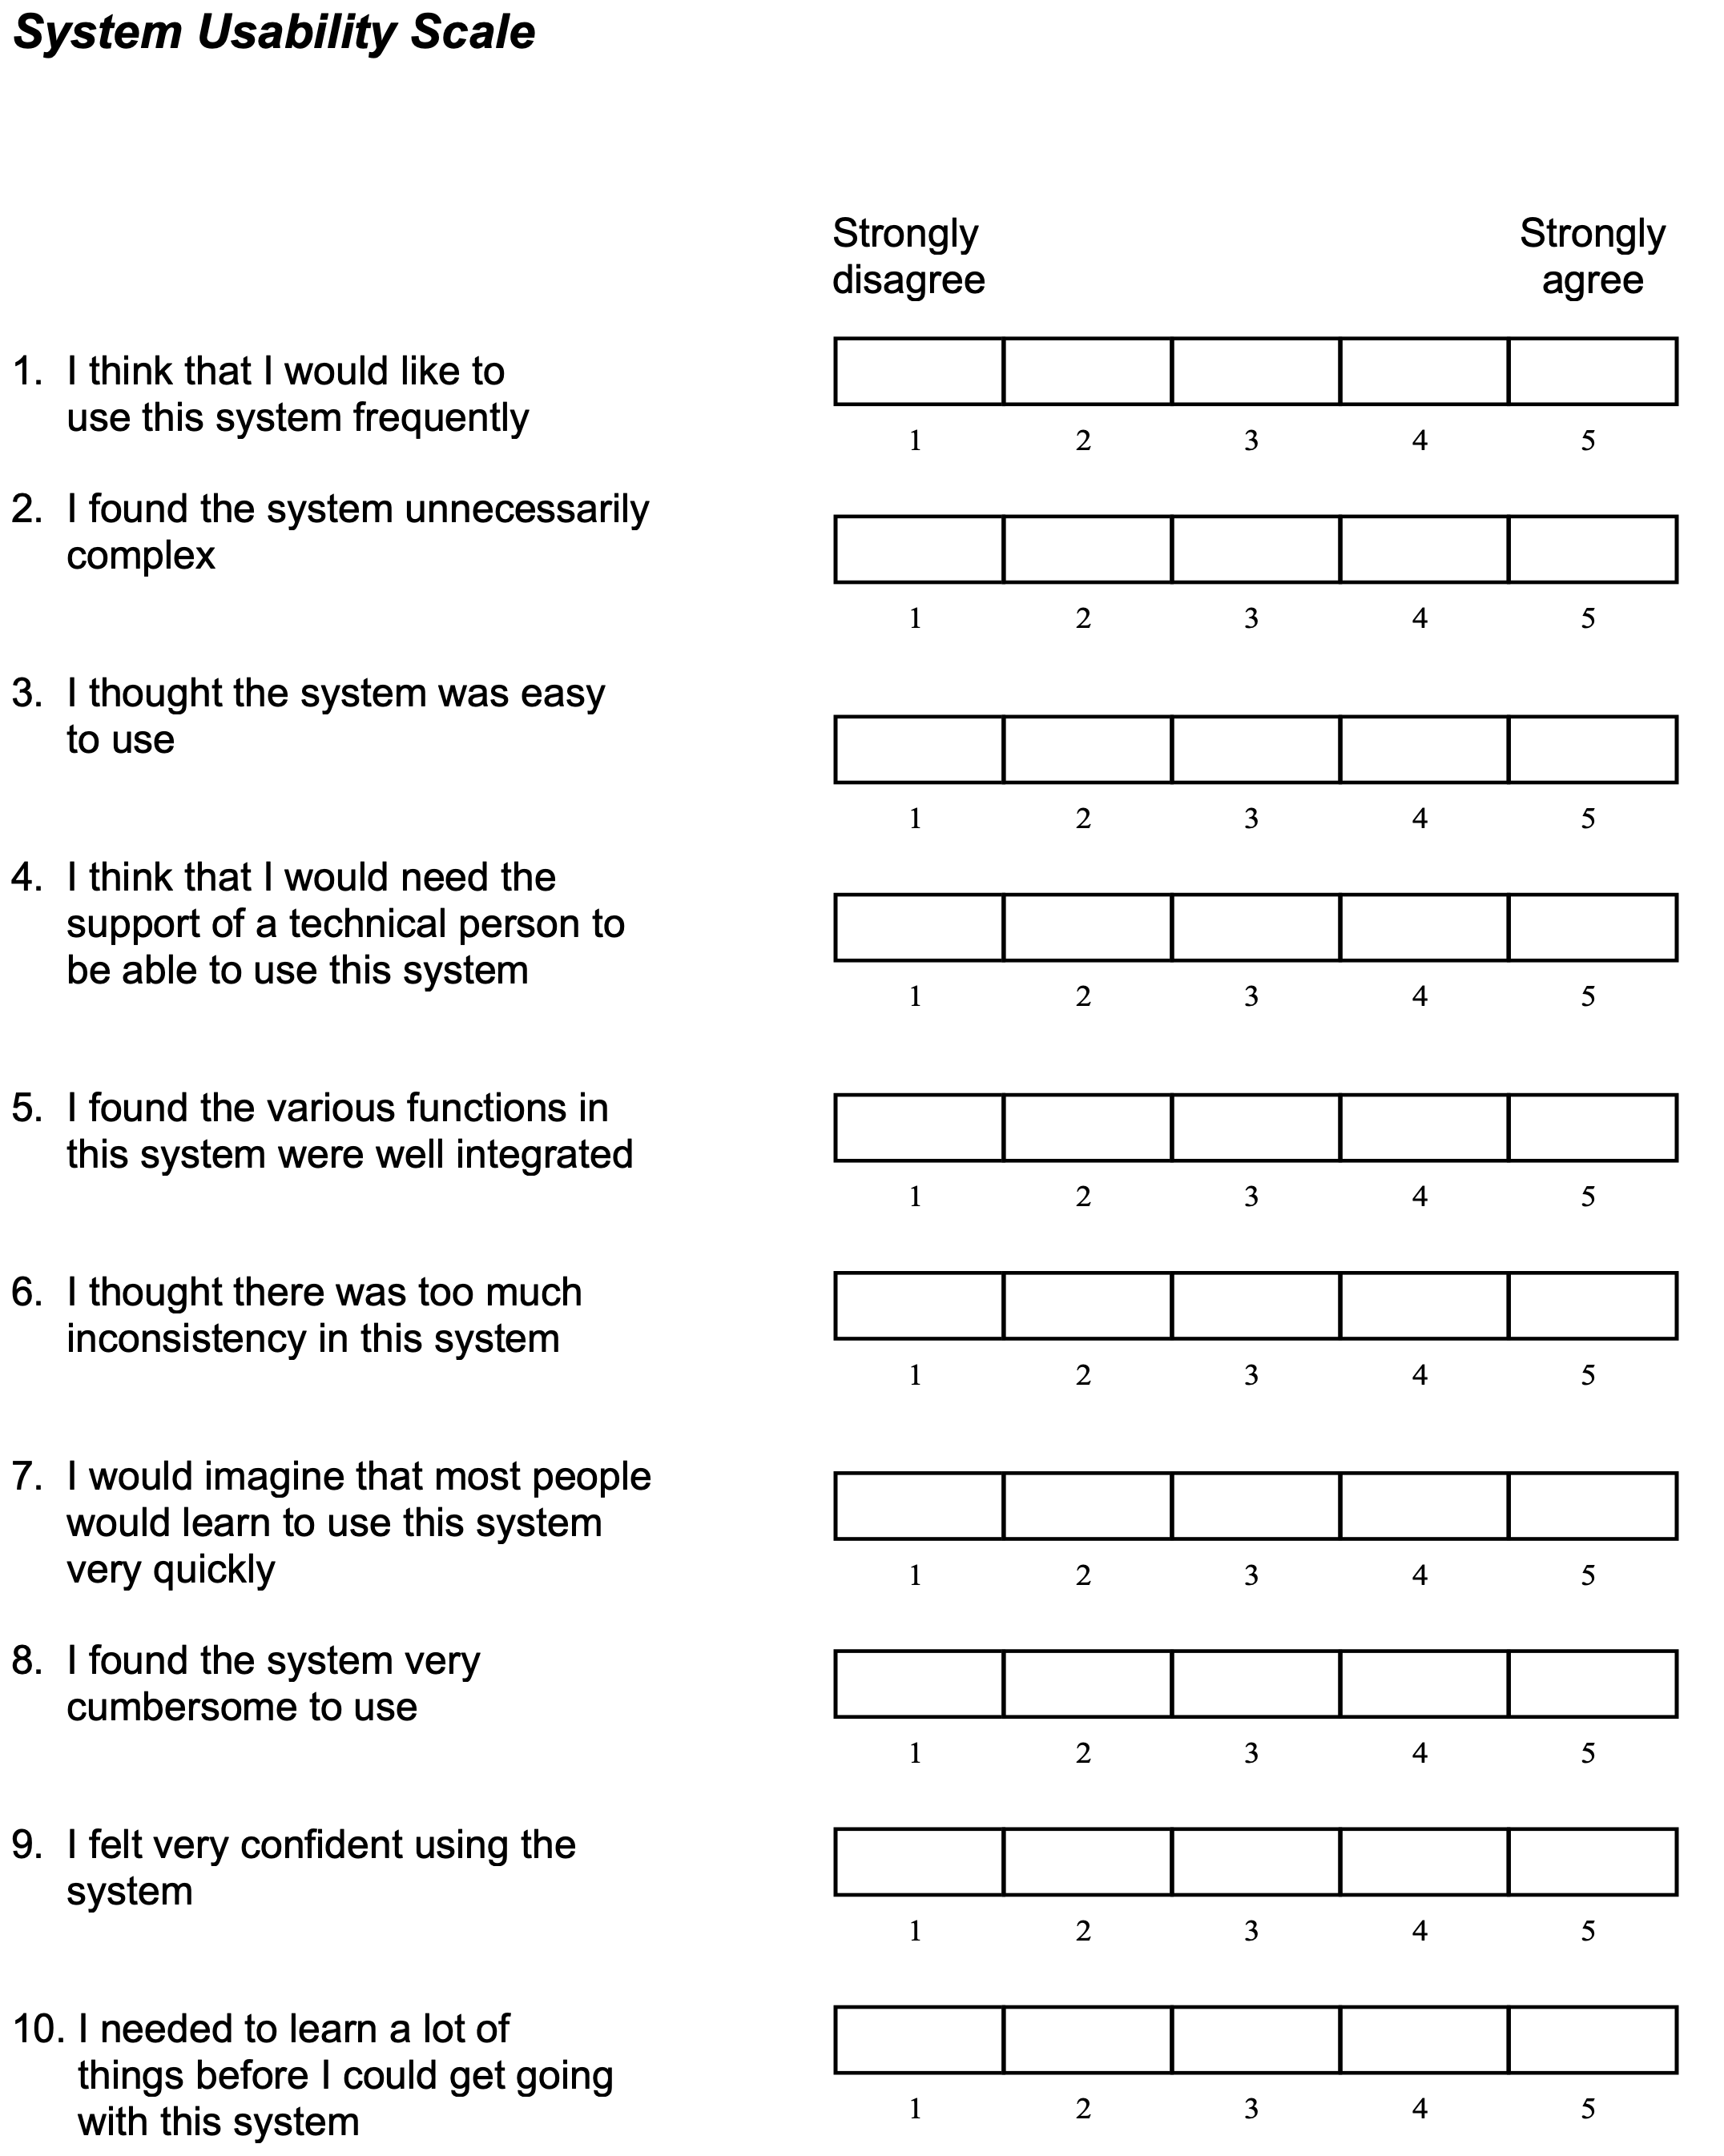
\includegraphics[width=0.7\linewidth]{figures/SUS}
	\caption{System Usability Scale}
	\label{fig:sus}
\end{figure}
